\documentclass{article}

%All LaTeX documents have a ``preamble'' that includes the packages and macros needed to make the document compile. The file `PomonaLgcsFormatting.tex' includes the preamble for this template. You can see it in the file list on the left frame of your screen, and this document is instructed to use it with the \input{} command below.

\input{PomonaLgcsFormatting}

\title{Pomona Linguistics: Quick Reference Guide for LaTeX}
\author{Michael Diercks and Franny Brogan}
\date{\today}

\begin{document}

\maketitle

\begin{abstract}

Here is where you write the abstract of the paper.

\end{abstract}

\vspace{-5mm} %Just pretend this isn't here we couldn't fit the table of contents on one page smh 

%Also, Franny had to google smh to learn what it means

%When you are editing this project to start writing your paper, just delete or comment out the table of contents, or keep it if you like seeing an outline generated of what you are writing. To see what a ``comment'' is, read the introduction below!

\tableofcontents

\section{Introduction}

Read the formatted document on the right of the screen, then look to the left to see the code that generated it! %The exclamation mark here shows how excited we are about LaTeX.

\subsection{What is \LaTeX?}

\LaTeX{} is a typesetting program that takes a text document (with the file type .tex) and converts it to a typeset document that can be easily made into a PDF. In Overleaf, the .tex document is on the left side of your screen and the typeset document is on the right, which can be downloaded as a PDF using the `Download PDF' button  right at the top of the preview.

In many ways \LaTeX{} is like familiar word processors (like Microsoft Word or Google Docs) because it is a typesetting program that takes input via a keyboard and produces a document that can be printed on paper. There are important differences, though. When using \LaTeX{} you directly annotate your text with commands that tell the program how to format the text. So if you want to write something in \textit{italics} you write \verb|\textit{italics}|, and if you want something \textbf{bolded} you write \verb|\textbf{bolded}|. \LaTeX{} then converts that `code' into what looks like italics and bold. In this Overleaf template, you can look at the .tex file itself to see what commands (`code') is used to create different kinds of formatting. 

%In the paragraph above, the command \verb|stuff| is from the package ``verbatim'' which prints whatever is written inside the |vertical lines| even if it is a command that usually does something in LaTeX. Just in case you were wondering what that command is.

\subsection{What is this document?}

This is a Quick Reference Guide (\href{https://www.overleaf.com/latex/templates/pomona-linguistics-quick-reference-guide/jthrqbrktmrd}{published as an Overleaf template}) for writing papers in \LaTeX{} for courses in Linguistics at Pomona College.\footnote{This Quick Reference Guide and the \href{https://www.overleaf.com/latex/templates/pomona-linguistics-latex-template/bvdxdtpwysnd}{corresponding Paper Template} were written by Michael Diercks and Franny Brogan. Diercks' original \LaTeX{} teaching materials were created with assistance from Claire Halpert, Nico Baier, Jason Zentz, Maddy Bossi, and Michael Clausen.} It serves two purposes: first, it provides examples of formatting you need to write papers in Phonology, Syntax, and Semantics/Pragmatics using \LaTeX, such as trees, numbered examples, etc. Second, if you have opened this as an Overleaf template, a copy of this project is now in your Overleaf account, and you can now edit this document itself to be an actual paper that you write. This means there is no setup required, you can just erase this text and start typing your own paper, or use this document to practice and see what changes your edits make.\footnote{This also means you will probably want to rename the document - you can do this by hovering your cursor over the title ``Pomona Linguistics Quick Reference Guide' at the top of this page, and then clicking on the pencil icon that appears to the right of the title. You can also rename the PomLingQuickReference.tex file in the leftmost panel by clicking on the down arrow.} Designing a \LaTeX{} project from scratch can be difficult; the point of this template is that this is already done for you, you can just start writing. Our \href{https://www.overleaf.com/latex/templates/pomona-linguistics-latex-template/bvdxdtpwysnd}{Paper Template} offers the same advantages without this (long) explanatory document.

\begin{itemize}

\item Don't worry about breaking anything - you can always open the template link again to see this initial version again. So edit away!

%Mess with the text in the .tex document right here and see what happens when you Recompile (the green button at the top left of the PDF viewer).

\item \textbf{Overleaf pro-tip}: if you want to find a location in the .tex document where the commands are written for what you are seeing in the preview on the right side of your screen, just double-click on the text in the preview and it will take you to the relevant portion of the .tex document.

\item Try this here - doubled click on this sentence in the preview and take a peek at where the cursor moved to in the .tex document to the left of this preview, to see what a ``comment'' is using the \% symbol. 

%As you can see, using the percentage symbol "%" creates a ``comment," i.e. something that appears in the .tex document, but which does not compile, and therefore has no effect on the document being produced. It's a handy way to write yourself notes. This does mean that if you ever want to use a % symbol that is not for a comment, you have to add a backslash in front of it to tell LaTeX that you don't mean for it to be a comment, like we did in the bullet point above.

%If you want to comment out a bunch of stuff at once in Overleaf, highlight it and Press Cmd-/ (or, Ctrl-/ on a PC). This will but a % in front of every line. It is a very handy tool when looking for errors, a process of elimination can help you find an error that is hiding from you.

\end{itemize}

\subsection{Some ways to work in \LaTeX}

Another difference between apps like Microsoft Word/Google Docs and \LaTeX{} is that \LaTeX{} is more similar to the code that makes Word/Google Docs function, rather than Word itself. \LaTeX{} doesn't come with a user interface, and instead people have created many different sorts of apps to access and use \LaTeX. 

\begin{itemize}

\item \textbf{RECOMMENDED}: Overleaf (\url{https://www.overleaf.com}) is a cloud-based \LaTeX{} editor that makes it quicker and easier to start writing in \LaTeX. Full access requires a paid subscription, but the free accounts  are  sufficient for most student work. If you are reading this template in Overleaf, you have already found your way here. If somehow you just found this document as a PDF and haven't found the Overleaf template, \href{https://www.overleaf.com/latex/templates/pomona-linguistics-quick-reference-guide/jthrqbrktmrd}{click here} to open this document in Overleaf. 

\item The \href{http://www.tlhiv.org/ltxpreview/}{online \LaTeX{} previewer} is restricted in what it can do, but if you are just drawing some basic trees or equations it is a quick-start way to start working with \LaTeX{}. The previewer allows you to preview what you wrote and download the images (or screenshot them), which can be inserted into a document you are working on in Microsoft Word or Google Docs.\footnote{That said, if you are writing your Syntax and/or Phonology papers in Google Docs, it is highly recommended that you switch to an application that is more suited to the task, e.g. Microsoft Word or \LaTeX{} in Overleaf. Pomona College students can \href{https://pomona.onthehub.com/WebStore/OfferingDetails.aspx?o=7479a671-aa7d-e511-9411-b8ca3a5db7a1}{access Microsoft Word for free.}} There are other similar applications (often referred to as equation editors) that are available online or downloadable for Mac/PC. Diercks has \href{http://pages.pomona.edu/~mjd14747/LateXpreviewer.pdf}{a set of instructions} for using the online \LaTeX{} previewer on \href{http://pages.pomona.edu/~mjd14747/tex.html}{his website}. 

\item If you want to install \TeX{} on your own computer, you can download the distribution for Windows here (\url{http://miktex.org}) and for Mac here (\url{http://www.tug.org/mactex/}). We do NOT recommend this for beginners. %No, seriously - unless you already know what you're doing please don't do this.

\end{itemize}

\subsection{\LaTeX{} tutorial}

In this document we don't provide a complete tutorial on \LaTeX{}: we don't need to, because Pedro Martins has already written a tutorial specifically for linguists that also happens to be the best beginner-oriented \LaTeX{} tutorial that we have ever found. You can find it here: \url{http://ptmartins.info/latex/}.

\subsection{Should I use \LaTeX{} to write my papers?}

The answer to this question is `maybe.' There are upsides to using \LaTeX{} for linguistics papers: it is easier to format complicated diagrams, it is easier to format interlinear glosses, it auto-numbers numbered examples, it can handle IPA fonts relatively well, it is much easier to create stable cross-references within your document. Many kinds of linguistics papers require complicated formatting that can be difficult (or impossible) to do in other applications. This is especially true for theoretical linguistics theses, which can become quite difficult to format. And especially for theses, some otherwise arduous tasks (like managing references) are relatively simple in \LaTeX{}.

That said, the major downside to using \LaTeX{} is that there is an initial learning curve. The existence of Overleaf (and resources like \href{https://www.overleaf.com/latex/templates/pomona-linguistics-quick-reference-guide/jthrqbrktmrd}{this guide} and \href{http://ptmartins.info/latex/}{Pedro Martin's tutorial}) make it more achievable to ascend the learning curve, but it is still not as simple as opening Google Docs and starting to type. Many people find the pay-offs to be worth the initial cost, but not everybody thinks so, often depending on what their particular formatting needs are (this is true among both professors and students). 

So, to be as clear as possible: there is \textbf{no inherent moral virtue} to working in \LaTeX{} vs. another application, and don't let anyone tell you otherwise. The main question is whether the application you are using serves the function that you need it to. We think the resources available make it achievable to write in \LaTeX{} for those who want to learn how (and, that this will be helpful to do the things we ask for in classes), but 1) it is not a requirement for any Pomona linguistics course, 2) Microsoft Word can be used to write all linguistics papers,\footnote{Google Docs less so, but you can probably eke it out.} and 3) we don't grade \LaTeX{} submissions higher than those written any other way.

\section{Some basic things you will want to know}

For a full tutorial, see \href{http://ptmartins.info/latex/}{Pedro Martin's tutorial}. But this section \textit{very} quickly outlines things you may want to know how to do to write papers for our courses at Pomona. 

\subsection{Font Sizes}

\noindent To change the font size for this entire document, you can go to the first line in the .tex document which gives the class of document \verb|\documentclass{article}| and add a different font size as an option, for example, you can change it to \verb|\documentclass[12pt]{article}| and recompile the document (the green button in the middle/top of your screen) and the document will be changed to 12pt font.  

\noindent Here is a collection of font-size commands to change the size of text in a specific location in your paper: 

\begin{itemize}
    \item \verb|\Huge| 
    \item \verb|\huge| 
    \item \verb|\LARGE| 
    \item \verb|\Large| 
    \item \verb|\large| 
    \item \verb|\normalsize| (default) 
    \item \verb|\small| 
    \item \verb|\footnotesize| 
    \item \verb|\scriptsize| 
    \item \verb|\tiny|
\end{itemize}

\noindent You can change the size of a font by {\huge putting it} inside brackets with {\Large one of these commands}, which can create a {\footnotesize lot of different font sizes}. Even {\tiny tiny ones}.


\subsection{Useful commands for text formatting, some that we built for you}
 \label{UsefulShortcuts}

The chart below is structured with the most general sorts of text formatting first, with linguistics-specific symbols/formatting at the bottom.

\ea 
	\begin{tabular}[t]{l l l}
		\toprule
		\textbf{Symbol/Annotation} & \textbf{Example} & \textbf{Code} \\ \midrule
		Ellipsis & \dots & \verb|\dots| \\
		Subscript & NP\subs{i} & \verb|NP\subs{i}| \\
		Superscript & NP\supers{i} & \verb|NP\supers{i}|\\ 
		Bold & \textbf{bold} & \verb|\textbf{bold}| \\
		Italic & \textit{italic} & \verb|\textit{italic}| \\
		Small Caps & \textsc{small caps} & \verb|\textsc{small caps}| \\
		Strikeout & \sout{strikeout} & \verb|\sout{strikeout}| \\
		Underline & \underline{underline} & \verb|\underline{underline}| \\
		circle something in text & \circled{something} & \verb|\circled{something}| \\
		Highlight something & \hl{something} & \verb|\hl{something}| \\
		Null & \nothing  & \verb|\nothing|\\
		Theta & \texttheta & \verb|\texttheta|  \\
		Phi & \ph & \verb|\ph| \\
		Hash & \# & \verb|\#| \\
		Label a left bracket & \Lb{VP} kick it ] & \verb|\Lb{VP}|\\
		Label a right bracket & [[kick\Rb{rt}ed\Rb{wd} & \verb|\Rb{rt},\Rb{wd}|\\
		Trace with index & \tr{k}  & \verb|\tr{k}| \\
		Bar-level node & X\1 & \verb|X\1| \\
		Head Node & X\0 & \verb|X\0| \\
		\bottomrule
	\end{tabular}
\z

\newpage 

\begin{itemize}

\item If you want to make a bulleted list, look at how this list is formatted in the .tex document using the ``itemize'' environment.

\item As you've already seen if you are paying attention to the .tex document on the left of your screen, sections, subsections, and sub-subsection are formatted with the commands \verb|\section{}|, \verb|\subsection{}|, and \verb|\subsubsection{}|, respectively.

\item Look at the .tex document to see how we bolded \textbf{this text} (and Overleaf has a shortcut to make it easy, Cmd-B on Macs, Ctrl-B on PCs). \textit{Similarly for italics}, Overleaf provides a shortcut (Cmd-I on Macs, Ctrl-I on PCs).

\item Write footnotes like this.\footnote{Hey, look at me, I'm a footnote.}

\end{itemize}

\subsection{How do I do X?}

You likely will wonder how to do something that seems mysterious in \LaTeX{} but that is so simple in other applications ... and it might possibly be driving you mad. Google is your friend. Type ``bulleted list in latex" into Google and you will quickly find instructions for a bulleted list, and you can use this method to find out how to do almost anything you need to do. That said, we've attempted to provide instructions for everything you need for Pomona Linguistics inside this \href{https://www.overleaf.com/latex/templates/pomona-linguistics-quick-reference-guide/jthrqbrktmrd}{Quick Reference Guide}.

\subsection{Heads up! Some potential pitfalls}

For all of \LaTeX{}'s conveniences, there are some annoyances that are puzzling until you figure them out. 

\begin{itemize}

    \item Quotation marks are easy to get wrong. You want them to display ``like this'' and not "like this," so use the grave accent symbol above your tab key to type front quotes. 

    \item Because a character like the percentage symbol \% actually means something in \LaTeX{} (it creates a comment), you can't just use a percentage symbol on its own to mean a percentage symbol. Instead, you have to put a backslash in front of it, like we did in in the previous sentence (check out the .tex document, and also \href{http://ptmartins.info/latex/#special-characters}{this note} about other similar characters).
    
    \item It is very easy to forget to put the end bracket on a command. So you might write this \verb|\hl{highlight this| instead of \hl{highlight this} (see the .tex) and your document will show an error. Thankfully Overleaf has warnings that pop up as you type if you have left a bracket open.
    
    \item Because it's possible to write code that won't compile, it is recommended to compile your document frequently while writing. This way, when you make a mistake you won't have pages and pages to sort through to find where the mistake is. The keystroke Cmd-S (on Mac) and Ctrl-S (on PC) will instruct Overleaf to Recompile, we suggest making it a habit to do this frequently while you write. %This makes things a lot easier, bc trying to find the broken piece of code somewhere inside your whole paper can be a real pain in the aaaaa  can we swear in here? probably shouldn't, eh 

\end{itemize}

\section{Numbered examples} \label{SectNumberedExs}

It is easy to create consecutively numbered examples; 

%\ea Watch the numbers change when you uncomment this and recompile!  \z 

\ea 
This example is auto-numbered - if you uncomment the example above and recompile, the numbering will change.
\z 

\noindent The \texttt{gb4e} package that we use for numbered examples allows for inter-linear glossing and translations: 

\ea 
\gll this is a language example \\
this is the morphological gloss \\
\glt `This is the translation.' 
\z 

\noindent  \texttt{gb4e} automatically aligns glosses with the language example (each white space means a different word). This is useful for non-English examples like the Lubukusu sentence in (\ref{BukusuNegation}): 

\ea \label{BukusuNegation}
\gll Peter se-a-la-ba a-kula sitabu ta. \hspace{2 in}  \textbf{Lubukusu} \\
Peter NEG-SA-TNS-be SA-buy book NEG \\
\glt `Peter will not be buying a book.'
\z

\noindent If you want multiple data examples to appear in one numbered example, you use the xlist environment, which you can see in the .tex document by double clicking on the example below in the preview: 

\ea \label{XlistExample}
\begin{xlist}

\ex This is the first example. 
\ex This is the second example. 

\end{xlist}

\z 

\noindent In many linguistics publications, \textit{all}  diagrams and data are presented as numbered examples (e.g. trees, tableaux, charts, sentences with interlinear glosses, data sets of words). You can see examples of this below for both phonology (\S \ref{SectPhonology}) and syntax (\S \ref{SectSyntax}). 

\section{Using cross-references} \label{SectCrossReferences}

It is useful to be able to refer your reader to different sections/examples in your paper: for example, we may want to tell you that examples (\ref{BukusuNegation}) and (\ref{XlistExample}) are built using \texttt{gb4e}, or that if you want to learn about fonts you should read \S \ref{SectFonts}. There are two components of a cross-reference in text: 

\begin{enumerate}    

\item You must label a particular section or example that you intend to refer to using the command \verb|\label{LabelName}| (where ``LabelName'' can be any text you choose to describe the example or section you are referring to), 
    
\item You must then use the \verb|\ref{LabelName}| command to create the cross-reference. 

\end{enumerate}

\noindent So if you look in the .tex at the example in (\ref{LabelSample}), you will see that we have chosen the label name ``LabelSample'' to identify the example. And if you look in the preceding sentence, you see an instance of using the \verb|\ref{}| command to create a cross-reference.

\ea \label{LabelSample}
A numbered example with a label 
\z

Notably, you can only use the \verb|\ref{LabelName}| command with labels that already exist somewhere in your paper - attempting to build a cross-reference to a label that does not exist will not stop your document from compiling, but it will result in a Yellow Warning from Overleaf next to the Recompile button, and it will result in question marks where the cross-reference ought to be, like this: (\ref{ToNothing}). %If you change the reference in the preceding sentence to (\ref{LabelSample}) instead of ``ToNothing,'' you will see the Yellow Warnings next to the Recompile button disappear. Which is of course very satisfying.

These cross-references are auto-generated every time you compile your document, so as your section/example numbers change as you write your paper, the cross-references update themselves. You will never have to renumber cross-references in your document again. %Unless you really LIKE renumbering cross-references; if so, then Google Docs is for you! 

\section{Fonts} \label{SectFonts}

\ea 
ðɪs ɪz haʊ tu raɪt ɪn ʔɑɪpijeɪ. (This is how to write in IPA.)
\z 

\noindent This template uses the package \texttt{fontspec}, which allows you to enter IPA symbols\footnote{In fact, fontspec is not specific to IPA and can typeset any Unicode symbols as long as the font you are using has those symbols.} directly into your .tex document and it appropriately typesets it when creating a PDF.\footnote{In order to compile, the \texttt{fontspec} package requires a specific compiler (\XeLaTeX{}), which is set in the Menu, which is next to the Overleaf logo at the top left of the screen. This is already done in this template so you don't have to do anything, but this note is here for any of you that start getting into the details of the template yourself.} This doesn't tell you how to type the IPA symbols in the first place, though. This requires a non-\LaTeX{} solution.

\begin{itemize}

    \item \textbf{Recommended}: \href{https://scripts.sil.org/cms/scripts/page.php?site_id=nrsi&id=uniipakeyboard}{SIL IPA keyboard} is downloadable on Mac and PC and gives you keystrokes for inserting IPA characters.\footnote{FYI there's no way to type a `\textrhookschwa' via this keyboard (as far as we know), so utilize one of the methods below.}
    
    \item \href{https://www.blugs.com/IPA/}{IPA Palette}
    
    \item \href{https://ipa.typeit.org}{Online IPA keyboard} where you can type symbols and then copy/paste them into your document
    
    \item The web app \href{http://detexify.kirelabs.org/classify.html}{detexify} is a handy tool that allows you to draw the symbol you want and it shows you what packages you need for that symbol, and what commands create it in \LaTeX{}.

\end{itemize}

\noindent If you \textbf{do} want a \LaTeX{}-based solution for creating IPA symbols (i.e. if you don't want to use the keyboards above), the \texttt{TIPA} package is the most commonly-used system for processing IPA symbols in \LaTeX{}. (\href{https://www.tug.org/TUGboat/tb17-2/tb51rei.pdf}{This document} is a good resource for the macro names (i.e. commands to draw a symbol) and shortcut characters you'll need if you want to use \texttt{TIPA}.) Crucially, \texttt{TIPA} phonetic symbols can be inputted in the following two ways (look at the .tex document to see how these are coded):
\begin{enumerate}
    \item Input macro names in the normal text environment, e.g., \dh\textsci s \textsci z ha\textupsilon\ tu ra\textsci t \textsci n \textglotstop\textscripta pije\textsci.
    \item Input macro names or \textit{shortcut characters} within the following groups or environment:
    \begin{itemize}
        \item \verb|\textipa{...}|, e.g., 
            \textipa{DIs Iz haU tu raIt In PApijeI}.
        \item \verb|{\tipaencoding ...}|, e.g., 
            {\tipaencoding DIs Iz haU tu raIt In PApijeI}.
        \item \verb|\begin{IPA} ... \end{IPA}|, e.g.,
            \begin{IPA}
            DIs Iz haU tu raIt In PApijeI.
            \end{IPA}
    \end{itemize}
\end{enumerate}

\noindent In our estimation, \texttt{TIPA} is functional if you have to write the occasional IPA character. But the learning curve for \texttt{TIPA} is not much different than the learning curve for the IPA keyboard (and it is harder to read the code in a document coded with \texttt{TIPA}, as you can see in the examples in the list above), so if you are frequently using IPA symbols, you will likely find it easier to learn the IPA keyboard linked to above.

\section{Basic tables}

Tables are super useful for formatting data and examples, but super counter-intuitive to produce in \LaTeX{} as compared to in Word/Google Docs. This section lays out the basics; see \S\ref{SectAdvTabs} for additional formatting tricks.

\subsection{General Structure of Tables}\label{SectGenTables}

The \texttt{tabular} environment is used to typeset tables. By default, \LaTeX{} tables are drawn without any vertical or horizontal lines and column width is predetermined; this means that any settings beyond these defaults must be defined by you. It sounds complicated, but it's actually pretty cool to have so much control over what your tables look like. Let's take a look at some simple examples.

Let's start with a basic 3x3 table with single horizontal and vertical borders. Take a look at the .tex doc to see how borders and column alignment (i.e. whether your text is aligned on the left, right, or in the center of the column) are specified. 

%The `|'s on the first line give us vertical borders, the `l's between them mean we want the text in those columns to be left-aligned (you can specify the alignment of text in each individual column with `l', `c' (center), or `r' (right)), and the \hline command creates a single horizontal border. To get the vertical line (|) press Shift-\. 

\begin{tabular}{|l|l|l|} 
\hline 
cell 1 & cell 2 & cell 3 \\ 
\hline
cell 4 & cell 5 & cell 6 \\
\hline
cell 7 & cell 8 & cell 9 \\
\hline
\end{tabular}

%Note that the contents of cells in a given row are separated by '&'. You should have the same number of '&' signs in every row, even if the contents of a given cell are blank (i.e. a blank cell will look like this: & &). Also note that new rows are created using '\\'. This is a more general LaTeX command you can use for manually starting a new line.

\noindent Now, here's a table that's identical to the one above, but with bolded column headers separated by a double horizontal line. Take a look at the code in the .tex document to see how it's different from the code that generated the table above. %You can generate as many horizontal lines as you'd like by duplicating the \verb|\hline| command. (And, similarly, you could also generate as many vertical lines as you wanted by duplicating the `|'s.)

\begin{tabular}{|l|l|l|}
\hline
\textbf{Header 1} & \textbf{Header 2} & \textbf{Header 3} \\
\hline\hline
cell 1 & cell 2 & cell 3 \\
\hline
cell 4 & cell 5 & cell 6 \\
\hline
cell 7 & cell 8 & cell 9 \\
\hline
\end{tabular}

\noindent Here's a table identical to the one above, but with text center-aligned.

\begin{tabular}{|c|c|c|}
\hline
\textbf{Header 1} & \textbf{Header 2} & \textbf{Header 3} \\
\hline\hline
cell 1 & cell 2 & cell 3 \\
\hline
cell 4 & cell 5 & cell 6 \\
\hline
cell 7 & cell 8 & cell 9 \\
\hline
\end{tabular}

\vspace{.2in} %In case you're interested, this command creates vertical space (the quantity of your choosing) in your doc.

\noindent Now let's add a title. %you can see this added a couple of things to the code: we are now using the ``table'' environment, and \caption*{} creates the title.  we added the command \centering which centers the table.

\begin{table}[h!] 
\caption*{I'm a table with at title}
\centering
\begin{tabular}{|c|c|c|}
\hline
\textbf{Header 1} & \textbf{Header 2} & \textbf{Header 3} \\
\hline\hline
cell 1 & cell 2 & cell 3 \\
\hline
cell 4 & cell 5 & cell 6 \\
\hline
cell 7 & cell 8 & cell 9 \\
\hline
\end{tabular}
\end{table}

\begin{table}[h!] 
\caption*{\large{I'm a table with a bigger title}}
\centering
\begin{tabular}{|c|c|c|}
\hline
\textbf{Header 1} & \textbf{Header 2} & \textbf{Header 3} \\
\hline\hline
cell 1 & cell 2 & cell 3 \\
\hline
cell 4 & cell 5 & cell 6 \\
\hline
cell 7 & cell 8 & cell 9 \\
\hline
\end{tabular}
\end{table}

\subsection{How to put a table inside a numbered example}

In many kinds of linguistics papers, tables are not formatted as a separate class of elements, but are instead simply another kind of numbered example. To do this, the only difference is that you include only the ``tabular'' environment (an ``environment'' is something that you ``begin'' and ``end'') and you omit the ``table'' environment. In addition, we added the option ``[t]'' to the tabular environment to align the top of the table with the numbered example.

\ea 

\begin{tabular}[t]{|c|c|c|} %The [t] here is what gets the alignment with the number correct
\hline
\textbf{Header 1} & \textbf{Header 2} & \textbf{Header 3} \\
\hline\hline
cell 1 & cell 2 & cell 3 \\
\hline
cell 4 & cell 5 & cell 6 \\
\hline
cell 7 & cell 8 & cell 9 \\
\hline
\end{tabular}

\z 

\subsection{How to auto-number your tables}
Alternately, you may want \LaTeX{} to automatically number your tables (not as a numbered example, but separately). You can do so by removing the `*' from the end of the \verb|\caption| command for any tables you want to be auto-numbered:

\begin{table}[h!] 
\caption{I'm an auto-numbered table} 
\centering
\begin{tabular}{|c|c|c|}
\hline
\textbf{Header 1} & \textbf{Header 2} & \textbf{Header 3} \\
\hline\hline
cell 1 & cell 2 & cell 3 \\
\hline
cell 4 & cell 5 & cell 6 \\
\hline
cell 7 & cell 8 & cell 9 \\
\hline
\end{tabular}
\end{table}

\section{Phonology Things} \label{SectPhonology}

\subsection{Derivations}
Now that you know how to make basic tables in the \texttt{tabular} environment, creating a derivation table is easy. Below is a template you can use as a foundation, applying what you learned in \S\ref{SectGenTables} to add or delete rows and columns as needed.

\ea Derivation table template

\begin{tabular}[t]{|c c c c l|}
\hline
`Gloss1' & `Gloss2' & `Gloss3' & `Gloss 4' & \textbf{Gloss} \\
/UF1/ & /UF2/ & /UF3/ & /UF4/ & \textbf{Underlying form of root}\\
\hline
 & & & & \textbf{Morphology}\\
\hline
 & & & & Rule name here\\
 & & & & Rule name here\\
\hline
 & & & &\textbf{Phonology}\\
\hline
 & & & & Rule name here\\
 & & & & Rule name here\\
 & & & & Rule name here\\
 & & & & Rule name here\\
\hline
[SF1] & [SF2] & [SF3] & [SF4] & \textbf{Surface form}\\
\hline
\end{tabular}
\z

\subsection{SPE Rules}
Typing up SPE-style rules in Word/Google Docs is a pain in the butt, even if you're using Bruce Hayes's handy `HowToBrackets' guide. Luckily, typesetting phonology rules in \LaTeX{} is relatively straightforward. This template uses the package \texttt{phonrule}, which employs the basic command \verb|\phon{target}{change}| and then builds on that for more complex rule types. Let's start simple and work our way up through the different rule formats you'll need to use in LGCS108 and beyond.

The command \verb|\phon{target}{change}| has two arguments: the first is the \textbf{target}, or input, of the rule, and the second is the \textbf{change}, or output. Let's say we have a rule that raises /e/ to [i]. Here, `/e/' is our \textbf{target} and `[i]' is our \textbf{change} (double-click on the rule below to see the code for it):

\phon{e}{i}

Now, let's say this rule only applies in a particular \textbf{environment}, or context. We'll need to add an \textbf{environment} to our rule, which we can do by modifying our command and adding a third (and sometimes a fourth) argument. There are three distinct commands you can use when you want to add an environment to your rule; which one you choose depends on \textit{where you want your environment to appear with respect to the place holder line (i.e., underscore)}: \verb|\phonr|, \verb|\phonl|, and \verb|\phonb|.
\begin{itemize}
    \item \verb|\phonl{target}{change}{environment}| will place your environment \textbf{to the left} of your place holder line: \phonl{e}{i}{u}
    \item \verb|\phonr{target}{change}{environment}| will place your environment \textbf{to the right} of your place holder line: \phonr{e}{i}{]\subs{word}}
    \item \verb|\phonb{target}{change}{left environment}{right environment}| will place the two components of your environment \textbf{on either side} of your place holder line: \phonb{e}{i}{u}{\Rb{word}}
\end{itemize}

Now, what if we want to write some or all parts of our rule using \textbf{feature specifications} instead of IPA symbols? The \verb|\phonfeat[]{}| command allows you to insert feature matrices into your rules using the same argument structure we saw above. Let's take a look at an example:

\ea \label{EngAspRule}
English Aspiration Rule: 
\phonl{\phonfeat[c]{-voice\\-delayed release}}
{[+spread glottis]}
{\Lb{word}} 
\z

\noindent Keep in mind that you an use the \verb|\phonfeat[]{}| command to insert feature matrices of any size into any part of your rule (the target, change, and/or environment) following the format presented in example (\ref{EngAspRule}) above.

As you may know, the English Aspiration Rule in (\ref{EngAspRule}) is incomplete; we need to add an additional environment. For rules that have more than one environment, we can add \textbf{curly brackets} to the environment of our rule. As far as we know, the \texttt{phonrule} package only allows you to add a single (open) curly bracket. Double click on rule in (\ref{EngAspRule}) to check out the code in the .tex document.

\ea \label{EngAspRuleRev}
English Aspiration Rule (revised): 
\phonc
{\phonfeat[c]{-voice\\-delayed release}}
{[+spread glottis]}
{\oneof[l]{\Lb{word}\phold \\ 
\Lb{\textsigma}\phold \phonfeat{+syllabic \\ +stress}}}
\z

%In the code above, the '\oneof[l]{}' command gives us an open curly bracket containing left-aligned text. Change the 'l' to 'r' or 'c' to change the text alignment. The `\phold' command manually creates a place holder line.

\noindent For the purposes of course papers and the like, the single-bracket version is probably fine, although you may want to check with your instructor. For more advanced \LaTeX{} users who want to include both left and right curly brackets, there's a makeshift way to do so in math mode; see the example below:

\ea \label{EngAspRuleRev2}
English Aspiration Rule (revised): 
\[ %go into math mode
\phonc
{\phonfeat[c]{-voice\\-delayed release}}
{[+spread glottis]}
{\oneof[l]{\Lb{word}\phold \\ 
\Lb{\textsigma}\phold \phonfeat{+syllabic \\ +stress}}}
\Bigg\}
\] %exit math mode
\z

\noindent This work-around isn't ideal--particularly because the opening and closing curly brackets are of slightly different sizes--but should suffice for your purposes.

\subsection{Phonemicization diagrams}\label{SectPhonDia}
For phonemicization diagrams, this template uses the \texttt{TikZ} package, which is a general tool for creating graphic elements in \LaTeX{}. Once you understand the basic structure of these diagrams, adding additional tiers, changing the information conveyed in your tier(s), and modifying association lines is fairly simple. 

 As you'll see in the .tex document, we're simply creating a series of ``nodes", naming them, positioning them in relation to one another using (x,y) coordinates, and then specifying what text each node should contain. Once each node has been named, we use the \verb|\draw| command to draw association lines between the nodes of our choice. Below are three sets of phonemicization diagrams of varying complexities so you can see how this works:

%You can adjust the (x,y) coordinates below and see the nodes move around, which will help you get a sense of how to control positioning of nodes. Be sure you understand the simple ones before moving to the complex ones.

\ea A simple set of phonemicization diagrams

\begin{tikzpicture}
%phoneme tier
\node (p1) at (1.5,1) {/b/};
\node (p2) at (4.5,1) {/d/};
%allophone tier
\node (a1) at (1,0) {[β]};
\node (a2) at (2,0) {[b]} ;
\node (a3) at (4, 0) {[ð]};
\node (a4) at (5, 0) {[d]} ;
%association lines
\draw (p1) -- (a1);
\draw (p1) -- (a2);
\draw (p2) -- (a3);
\draw (p2) -- (a4);
\end{tikzpicture}
\z

\ea A slightly more complex set of phonemicization diagram

\begin{tikzpicture}
%phoneme tier
\node (p1) at (1.5,1) {/b/};
\node (p2) at (4.5,1) {/d/};
\node (p3) at (7.5,1) {/ɡ/};
%allophone tier
\node (a1) at (1,0) {[β]};
\node (a2) at (2,0) {[b]} ;
\node (a3) at (4, 0) {[ð]};
\node (a4) at (5, 0) {[d]} ;
\node (a5) at (7, 0) {[ɣ]};
\node (a6) at (8,0) {[ɡ]};
%association lines
\draw (p1) -- (a1);
\draw (p1) -- (a2);
\draw (p2) -- (a3);
\draw (p2) -- (a4);
\draw (p3) -- (a5);
\draw (p3) -- (a6);
%environment tier
\node (e1) at (1,-.5) {V\phold V};
\node (e2) at (2.25,-.5) {\textit{elsewhere}};
\node (e3) at (4,-.5) {V\phold V};
\node (e4) at (5.25,-.5) {\textit{elsewhere}};
\node (e5) at (7,-.5) {V\phold V};
\node (e6) at (8.25,-.5) {\textit{elsewhere}};
\end{tikzpicture}
\z

\ea A very complex set of phonemicization diagram

\begin{tikzpicture}
%phoneme tier
\node (p1) at (1,1) {/i/};
\node (p2) at (3,1) {/u/};
\node (p3) at (7,1) {/ɛ/};
\node (p4) at (9,1) {/a/};
\node (p5) at (13,1) {/o/};
%allophone tier
\node (a1) at (1,0) {[i]};
\node (a2) at (3,0) {[u]};
\node (a3) at (5,0) {[$\emptyset$]};
\node (a4) at (7,0) {[ɛ]};
\node (a5) at (9,0) {[a]};
\node (a6) at (11,0) {[ə]};
\node (a7) at (13,0) {[o]};
%association lines
\draw (p1) -- (a1);
\draw (p1) -- (a3);
\draw (p2) -- (a2);
\draw (p2) -- (a3);
\draw (p3) -- (a4);
\draw (p3) -- (a6);
\draw (p4) -- (a5);
\draw (p4) -- (a6);
\draw (p5) -- (a7);
\draw (p5) -- (a6);
%environment tier
\node (e1) at (1,-.5) {\textit{elsewhere}};
\node (e2) at (3,-.5) {\textit{elsewhere}};
\node (e3) at (5,-.5) {\phold\Rb{word}};
\node (e4) at (7,-.5) {\textit{elsewhere}};
\node (e5) at (9,-.5) {\textit{elsewhere}};
\node (e6) at (11,-.5) {[-stress]};
\node (e7) at (13,-.5) {\textit{elsewhere}};
\end{tikzpicture}
\z

\noindent We recommend starting with your most ``basic" tier (that is, the tier whose spatial positioning you're most sure of) and then positioning your other tiers accordingly. We like to start with the allophone tier and then position the corresponding phonemes and environments around it.  

%Note that we've used the \phold command from the phonrule package in the environment for [∅]. 

You can embed any component from the \texttt{phonrule} package in the \textit{tikzpicture} environment when drawing phonemicization diagrams, such as feature matrices, as in (\ref{RuleNeut}).

\ea Neutralization of /t/ and /d/ in English \label{RuleNeut}

\begin{tikzpicture}
%phoneme tier
\node (p1) at (1,1) {/t/};
\node (p2) at (7,1) {/d/};
%allophone tier
\node[anchor=base] (a1) at (1,0) {[t]};
\node[anchor=base] (a2) at (4,0) {[ɾ]};
\node[anchor=base] (a3) at (7,0) {[d]};
%association lines
\draw (p1) -- (a1);
\draw (p1) -- (a2);
\draw (p2) -- (a2);
\draw (p2) -- (a3);
%environment tier
\node (e1) at (1,-1) {\textit{elsewhere}};
\node (e2) at (4,-1) {\phold\phonfeat[c]{+syllabic\\-stress}};
\node (e3) at (7,-1) {\textit{elsewhere}};
\end{tikzpicture}
\z

\subsection{Autosegmental diagrams}\label{autoseg}
There are various packages you an use to draw diagrams with autosegmental tiers in \LaTeX{}. More advanced users may be interested in exploring the \texttt{pst-asr} package, which was designed to be used by linguists to typeset autosegmental representations (and generally renders them more aesthetically-pleasing than what you'll see here). Package contents can be found \href{https://ctan.org/tex-archive/graphics/pstricks/contrib/pst-asr/}{here}. 

For the sake of simplicity, this template typesets autosegmental diagrams using the \texttt{TikZ} package, which we introduced in \S\ref{SectPhonDia}. Let's start with a basic example that illustrates the syllabic division of the word \textit{phonology}, [fə.nɑ.lə.dʒi].

\ea Syllable associations for \textit{phonology}, [fə.nɑ.lə.dʒi]

\begin{tikzpicture}
%syllable tier
\node (s1) at (1,0) {\textsigma} ; 
\node (s2) at (2,0) {\textsigma} ; 
\node (s3) at (3,0) {\textsigma} ;
\node (s4) at (4,0) {\textsigma} ;
%segment tier
\node[anchor=base] (c1) at (0.5,-1) {f} ; 
\node[anchor=base] (v1) at (1,-1) {ə} ;
\node[anchor=base] (c2) at (1.5,-1) {n} ;
\node[anchor=base] (v2) at (2,-1) {ɑ} ;
\node[anchor=base] (c3) at (2.5,-1) {l} ;
\node[anchor=base] (v3) at (3,-1) {ə} ;
\node[anchor=base] (c4) at (3.5,-1) {dʒ} ;
\node[anchor=base] (v4) at (4,-1) {i} ;
%association lines
\draw (s1) -- (c1) ;
\draw (s1) -- (v1) ;
\draw (s2) -- (c2) ;
\draw (s2) -- (v2) ;
\draw (s3) -- (c3) ;
\draw (s3) -- (v3) ;
\draw (s4) -- (c4) ;
\draw (s4) -- (v4) ;
\end{tikzpicture} %close tikzpicture environment
\z

%The "anchor=base" option used above vertically aligns the nodes so that they appear at the same height.

\noindent Now, using the \verb|\stackanchor{}{}| command in the \texttt{stackengine} package, we can add a \textbf{stress tier} under our syllable nodes to show that [fə.nɑ.lə.dʒi] has antepenultimate stress. Notice that we've also shifted all our nodes (except for the left-most group) over .5 on the x-axis to make room for the stress tier:

\ea Syllable and stress associations for \textit{phonology}, [fə.ˈnɑ.lə.dʒi]

\begin{tikzpicture}
%syllable tier
\node (s1) at (1,0) {\stackanchor{\textsigma}{[-stress]}} ;
\node (s2) at (2.5,0) {\stackanchor{\textsigma}{[+stress]}} ;
\node (s3) at (4,0) {\stackanchor{\textsigma}{[-stress]}} ;
\node (s4) at (5.5,0) {\stackanchor{\textsigma}{[-stress]}} ;
%segment tier
\node[anchor=base] (c1) at (0.5,-1) {f} ;
\node[anchor=base] (v1) at (1,-1) {ə} ;
\node[anchor=base] (c2) at (2,-1) {n} ;
\node[anchor=base] (v2) at (2.5,-1) {ɑ} ;
\node[anchor=base] (c3) at (3.5,-1) {l} ;
\node[anchor=base] (v3) at (4,-1) {ə} ;
\node[anchor=base] (c4) at (5,-1) {dʒ} ;
\node[anchor=base] (v4) at (5.5,-1) {i} ;
%association lines
\draw (s1) -- (c1) ;
\draw (s1) -- (v1) ;
\draw (s2) -- (c2) ;
\draw (s2) -- (v2) ;
\draw (s3) -- (c3) ;
\draw (s3) -- (v3) ;
\draw (s4) -- (c4) ;
\draw (s4) -- (v4) ;
\end{tikzpicture}
\z

\noindent Now let's build on this foundation, adding \textbf{structure above the syllable}. Suppose we want to show stress, syllable structure, and word division for the phrase \textit{go, Dodgers!}, [ˈɡoʊ.ˈdɑ.dʒ\textrhookschwa z]:

\ea Word, syllable, and stress associations for \textit{go, Dodgers!}, [ˈɡoʊ.ˈdɑ.dʒ\textrhookschwa z]

\begin{tikzpicture}
%word tier
\node (w1) at (1,1) {word};
\node (w2) at (3.25,1) {word};
%syllable tier
\node (s1) at (1,0) {\stackanchor{\textsigma}{[+stress]}} ;
\node (s2) at (2.5,0) {\stackanchor{\textsigma}{[+stress]}} ;
\node (s3) at (4,0) {\stackanchor{\textsigma}{[-stress]}} ;
%segment tier
\node[anchor=base] (c1) at (0.5,-1) {ɡ} ;
\node[anchor=base] (v1) at (1,-1) {oʊ} ;
\node[anchor=base] (c2) at (2,-1) {d} ;
\node[anchor=base] (v2) at (2.5,-1) {ɑ} ;
\node[anchor=base] (c3) at (3.5,-1) {dʒ} ;
\node[anchor=base] (v3) at (4,-1) {\textrhookschwa} ;
\node[anchor=base] (c4) at (4.5,-1) {z} ;
%association lines
\draw (s1) -- (c1) ;
\draw (s1) -- (v1) ;
\draw (s2) -- (c2) ;
\draw (s2) -- (v2) ;
\draw (s3) -- (c3) ;
\draw (s3) -- (v3) ;
\draw (s3) -- (c4) ;
\draw (w1) -- (s1) ;
\draw (w2) -- (s2) ;
\draw (w2) -- (s3) ;
\end{tikzpicture}
\z

\noindent To build more tiers, simply add additional sets of nodes and association lines accordingly.

Finally, using the \texttt{TikZ} package, we can follow the procedure outlined above to create a tier for \textbf{tonal autosegments}. Below we see the hypothetical underlying form /cedeari/ with its tonal associations:

\ea Underlying tonal associations for /cedari/

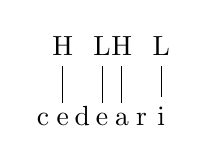
\begin{tikzpicture}
%tone tier (4 tones)
\node (t1) at (1.25,1) {H};
\node (t2) at (1.75,1) {L};
\node (t3) at (2,1) {H};
\node (t4) at (2.5,1) {L};
%segment tier (7 segments)
\node[anchor=base] (c1) at (1,0) {c} ;
\node[anchor=base] (v1) at (1.25,0) {e} ;
\node[anchor=base] (c2) at (1.5,0) {d} ;
\node[anchor=base] (v2) at (1.75,0) {e} ;
\node[anchor=base] (v3) at (2,0) {a} ;
\node[anchor=base] (c3) at (2.25,0) {r} ;
\node[anchor=base] (v4) at (2.5,0) {i} ;
%association lines (4)
\draw (t1) -- (v1);
\draw (t2) -- (v2);
\draw (t3) -- (v3);
\draw (t4) -- (v4);
\end{tikzpicture}
\z

\noindent It's recommended that you play around with spacing and node placement here. Similar to the procedure laid out in \S\ref{SectPhonDia}, we like to start by anchoring the segments themselves and subsequently placing the tones to match the x values for their corresponding vowels. Note that one advantage of using the \texttt{TikZ} package for autosegmental diagrams is the ease with which you can control your association lines. For example, let's say we have a Syncope rule that deletes the second /e/ from the underlying form above, leaving its `L' tone unassociated. We simply \textbf{delete or comment out the /e/ node} as well as \textbf{its tonal association line}:

\ea Tonal associations for /cedari/ after Syncope applies

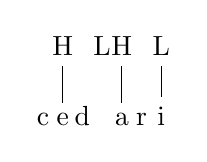
\begin{tikzpicture}
%tone tier (4 tones)
\node (t1) at (1.25,1) {H};
\node (t2) at (1.75,1) {L};
\node (t3) at (2,1) {H};
\node (t4) at (2.5,1) {L};
%segment tier (now only 6 segments)
\node[anchor=base] (c1) at (1,0) {c} ;
\node[anchor=base] (v1) at (1.25,0) {e} ;
\node[anchor=base] (c2) at (1.5,0) {d} ;
\node[anchor=base] (v3) at (2,0) {a} ;
\node[anchor=base] (c3) at (2.25,0) {r} ;
\node[anchor=base] (v4) at (2.5,0) {i} ;
%association lines (now only 3 lines)
\draw (t1) -- (v1);
\draw (t3) -- (v3);
\draw (t4) -- (v4);
\end{tikzpicture}
\z

\noindent Now imagine that, after Syncope applies, a Reassociation rule associates stray tones with the following vowel. We can show the reassociation of `L' by connecting it to the [a] segment:

\ea Tonal associations for /cedari/ after Syncope and Reassociation


\begin{tikzpicture}
%tone tier 
\node (t1) at (1.25,1) {H};
\node (t2) at (1.75,1) {L};
\node (t3) at (2,1) {H};
\node (t4) at (2.5,1) {L};
%segment tier
\node[anchor=base] (c1) at (1,0) {c} ;
\node[anchor=base] (v1) at (1.25,0) {e} ;
\node[anchor=base] (c2) at (1.5,0) {d} ;
\node[anchor=base] (v3) at (2,0) {a} ;
\node[anchor=base] (c3) at (2.25,0) {r} ;
\node[anchor=base] (v4) at (2.5,0) {i} ;
%association lines (back to 4)
\draw (t1) -- (v1);
\draw (t2) -- (v3);
\draw (t3) -- (v3);
\draw (t4) -- (v4);
\end{tikzpicture}
\z

\subsection{Tableaux}
While you can certainly make beautiful Optimality-Theoretic tableaux in the \texttt{tabular} environment, the \texttt{ot-tableau} package makes this task a little bit easier. The \texttt{ot-tableau} package uses the \texttt{tableau} environment, which functions similarly to the \texttt{tabular} environment. Here's a simple tableau with three candidates and three constraints with a known ranking, as indicated by the solid vertical lines between constraints:

\ea Simple tableau with known constraint ranking

\begin{tableau}{c|c|c} 
\inp{\ips{stap}} 
\const{*Complex} 
\const{Anchor-IO} 
\const{Contiguity-IO}
\cand{stap} \vio{*!} \vio{} \vio{} 
\cand[\Optimal]{sap} \vio{} \vio{} \vio{*}
\cand{tap} \vio{} \vio{*!} \vio{}
\end{tableau}
\z

%A few things to note here: 
    % 1. In the parameter in the first line of code, the `c's mean `constraint', not `center align'.
    %2. The input line is specified using the \inp command, and within that, the \ips command is used to render the text using TIPA and put it within slashes. If you don't want it to do this automatically, just get rid of the \ips command and add your slashes and IPA text manually.
    %3. The \Optimal command gives you the pointy finger.

Here's the same tableau, but with a dotted line separating the first and second constraints to indicate that the ranking relationship between these two constraints is unknown:

\ea Simple tableau with partially-known constraint ranking

\begin{tableau}{c:c|c}
\inp{\ips{stap}} 
\const{*Complex} 
\const{Anchor-IO} 
\const{Contiguity-IO} 
\cand{stap} \vio{*!} \vio{} \vio{} 
\cand[\Optimal]{sap} \vio{} \vio{} \vio{*} 
\cand{tap} \vio{} \vio{*!} \vio{}
\end{tableau}
\z


Finally, here's an example of a tableau where the incorrect constraint ranking gives us the wrong ``winner". The \bomb{} marks the candidate that wins (but shouldn't), and the \grimace{} marks the candidate that should win (but doesn't):

\ea Simple tableau with incorrect constraint ranking

\ShadingOn
\begin{tableau}{c|c|c}
\inp{\ips{stap}} 
\const{*Complex} 
\const{Contiguity-IO} 
\const{Anchor-IO} 
\cand{stap} \vio{*!} \vio{} \vio{} 
\cand[\grimace]{sap} \vio{} \vio{*!} \vio{} 
\cand[\bomb]{tap} \vio{} \vio{} \vio{*}
\end{tableau}
\z

\section{Syntax Things} \label{SectSyntax}


\subsection{Trees trees trees}

One of the biggest things syntacticians rely on \LaTeX{} for is drawing trees. This template uses the package \texttt{forest}, so to draw a tree in this template you use the \verb|\Forest{tree.in.here}| command. (look to the left at the .tex document for the code for the tree below)

\ea \label{FirstTree}
\Forest{
[VP
    []
    [V\1
        [V\0]
        [NP]
    ]
] 
}
\z 

\noindent The code for (\ref{FirstTree}) is formatted so that each level of the tree is indented separately. This is not necessary; the code for (\ref{FirstTreeCondensed}) has the same exact bracket structures, just with no line breaks or indents. You'll see in the preview that these trees are identical, despite the code in the .tex document being formatted differently.

\ea \label{FirstTreeCondensed}
\Forest{
[VP [] [V\1 [V\0] [NP] ] ] 
}
\z 

\noindent We recommend formatting your code something more like (\ref{FirstTree}) than (\ref{FirstTreeCondensed}), largely because as the trees get larger it can get tougher and tougher to interpret your code. We encourage you to try editing the trees above and see what happens! 

%%DO NOT INCLUDE EMPTY LINES IN THE CODE FOR THE TREE - As you can see, if you add an empty line to the trees above and attempt to recompile, you will get an error. Forest attempts to parse all lines so empty lines confuse it. 

You will notice in the tree above that because there is an empty branching node, the branches don't all go at precisely the same angle. There are spacing options you can invoke to adjust this, as in the example below, where the top node in the tree is specified as having ``nice empty nodes:'' 

\ea 
\Forest{
[VP, nice empty nodes
    []
    [V\1
        [V\0]
        [NP]
    ]
] 
}
\z 

\noindent This is really only helpful for a tree where there are empty branching nodes. We suspect many syntax students will prefer the nice empty nodes option when there are empty nodes ... but it can cause some messes with more complex trees, so there are times when it is advisable to simply live with some off-angle brackets. Please, please be willing to accept some mild imperfections in tree branch angles rather than spending hours and hours trying to fix it, at least for class papers. %it's just not worth it  

\noindent If you want to include text under a node, you include a line break (two backslashes) and add the text, as with the verb below. If you want to include a triangle, you include the desired text in brackets followed by the code ``, roof'' as seen below.

\ea \label{FullVpTree}
\Forest{
%for tree={s sep=10mm, inner sep=0, l-=3mm}
[VP 
    [DP [Maya, roof] ]
    [V\1 
        [V\0 \\ kick ]
        [DP [the ball, roof] ] 
    ] 
] 
}
\z 

%You'll notice in the code for the tree in (\ref{FullVpTree}) that there are some specific annotation for tree dimensions (sep, inner sep, etc) commented out. See \S \ref{AdvancedForest} for details about how this works. You can also uncomment it and see what happens.

\noindent Some larger tree skeletons are commented out immediately below this paragraph in case you want a template to work from for a larger tree. Remember, to (un)comment batches of text in Overleaf, highlight the text and press Cmd-/ (Mac) or Ctrl-/ (PC). 

% \ea 
% \Forest{
% [CP
%   []
%   [C\1
%         [C\0]
%         [TP 
%             []
%             [T\1 
%                 [T\0]
%                 [VP 
%                     []
%                     [V\1
%                         [V\1]
%                         [NP]
%                     ]
%                 ] 
%             ] 
%         ] 
%     ]
% ]
% }
% \z 

% \ea 
% \Forest{
% [CP, nice empty nodes
%   []
%   [C\1
%         [C\0]
%         [TP 
%             []
%             [T\1 
%                 [T\0]
%                 [VP 
%                     []
%                     [V\1
%                         [V\1]
%                         [NP]
%                     ]
%                 ] 
%             ] 
%         ] 
%     ]
% ]
% }
% \z 

Here's what a head-final tree looks like, where the difference is what you would expect: the node for the head follows the node for the complement of the head. 

\ea 
\Forest{
[CP, %nice empty nodes
  []
  [C\1
        [TP 
            [DP [subject, roof] ]
            [T\1 
                [VP 
                    []
                    [V\1
                        [DP [object, roof] ]
                        [V\0 \\ verb ]
                    ]
                ]
                [T\0]
            ] 
        ]
        [C\0]
    ]
]
}
\z 



\subsection{Annotating Trees}

\subsubsection{Boxes in Trees}

At times people find it useful to draw a box around a subtree. The clunky code attached to the VP node below makes that happen, which you can copy and paste into your paper if you want to draw a box in a tree. 

%The piece of code commented out below this comment is what draws the box - copy and paste it into your tree where you want it.

%tikz={\node [draw,fit to=tree]{};} 

\ea 
\Forest{
for tree={s sep=10mm, inner sep=0, l-=3mm}
[TP
    [DP\subs{k} [Maya, roof] ]
    [T\1
        [T\0 \\ will ]
        [VP, tikz={\node [draw,fit to=tree]{};} 
          [ \tr{k} ]
          [V\1 
              [V\0 \\ kick ]
              [DP [the ball, roof] ] 
          ] 
        ] 
    ]
]
}
\z 

\subsubsection{Arrows in Trees}

Arrows are drawn in a tree with the command \verb|\draw|. You must name specific nodes in your tree, and then you can draw an arrow from one node to the other in the last line of code in the tree. In the tree below we named the triangled DP ``SUBJ'' and the trace in Spec,VP as ``SpecVP,'' and then used those names in the command to draw the arrow, which is the last line of code in the tree. 

\ea \label{ArrowTree}
\Forest{
for tree={s sep=10mm, inner sep=0, l-=3mm}
[TP
    [DP\subs{k} [Maya, roof, name=SUBJ] ]
    [T\1
        [T\0 \\ will ]
        [VP 
          [ \tr{k}, name=SpecVP ]
          [V\1 
              [V\0 \\ kick ]
              [DP [the ball, roof] ] 
          ] 
        ] 
    ]
]
\draw[->] (SpecVP) to[out=south west,in=south] (SUBJ);
}
\z 

\noindent Please note, include arrows in a tree only when they serve to visually clarify the structure. They take extra time to draw, and traces/strikeout show the same exact information in a different notation. Be circumspect with how you spend your time here!

%The argument of draw is used to indicate the direction the arrow should be pointing: up [->], or down [<-], both [<->], or none [-]. 

\subsubsection{Spacing of Nodes in Trees} \label{NodeSpacingForest}

Forest will generally arrange the spacing around nodes for you, but it also allows you to specify it yourself. The ``s sep'' command controls horizontal spacing, ``l'' controls vertical spacing, and ``inner sep'' controls spacing around nodes. The tree in (\ref{AdvancedNodeEdits}) is identical in structure to the one above in (\ref{ArrowTree}), but we have commented out the commands defining the node spacing. Uncomment it, and change the numbers there, and then recompile the document to see what the effects on the tree are.

%Don't panic if you break the tree! Remember, you can always redownload this template if you need to go back to the initial state.

\ea \label{AdvancedNodeEdits}
\Forest{
%for tree={s sep=10mm, inner sep=0, l-=3mm}
[TP
    [DP\subs{k} [Maya, roof, name=SUBJ] ]
    [T\1
        [T\0]
        [VP 
          [ \tr{k}, name=SpecVP ]
          [V\1 
              [V\0 \\ kick ]
              [DP [the ball, roof] ] 
          ] 
        ] 
    ]
]
\draw[->] (SpecVP) to[out=south west,in=south] (SUBJ);
%You'll note in the `draw' command that you specify (with cardinal directions) which side of the nodes the arrow line comes in and out of. Change those to other directions (west, north west, etc) and recompile to see what the effects are.
}
\z 

There is a lot of other kinds of formatting of arrows and trees that may be of interest to syntax students: we have another Overleaf template (the \href{https://www.overleaf.com/latex/templates/arrows-for-syntax-diagrams-with-forest/xjyvcszgcspv}{Forest Arrows Explainer} that goes into much more detail for those who are interested.

\subsection{Linear structures with arrows} \label{SectLinearDiagrams}

At times it is also nice to be able to present a linear syntactic structure that shows movement without drawing a whole tree, as in (\ref{LinearExample}). If you are interested in these kinds of structures, see the \href{https://www.overleaf.com/latex/templates/arrows-for-syntax-diagrams-with-forest/xjyvcszgcspv}{Forest Arrows Explainer}.

\vspace{2em} %this adds vertical space above the example, bc drawing lines above the example takes space and it will overlap with the preceding paragraph otherwise. You can comment out the \vspace command to see what happens without it.

\ea \label{LinearExample}

\Lb{CP} \rnode{who2}{Who} \rnode{do2}{do} \Lb{TP} the children \rnode{do1}{\sout{do}} like to visit \rnode{who1}{\sout{who}} ? ] ] %the \rnode s have two arguments: the first is the name of the node and the second is the text that is shown.
\psset{linearc=3pt,nodesep=5pt} %this makes the arrows look pretty (rounded corners and not starting inside the words
\ncbar[angle=90]{<-}{who2}{who1} %this is the top arrow
\ncput*{wh-movement} %and this is the text on the top arrow. I'm pretty sure you just need to put the commands for the arrow and the text next to each other. No text necessary, this line can be deleted/commented out
\ncbar[angle=-90]{<-}{do2}{do1} %this is the bottom arrow, the minus sign did that
\ncput*{T-C-mov't} % this is the text on bottom  arrow. 
\z

\vspace{2em} 

\subsection{What if a tree/figure is too big for the page?}

Occasionally we run into issues where the tree we want to draw is too big to fit into the space on the page where we are putting it. There are a variety of ways that this can be dealt with in \LaTeX{}, but we recommend using \verb|\scalebox{number}{Tree/figure}|, where the number in the first argument of the command is the scale of the Tree (or other figure). In (\ref{BigTreeSample}) we drew a tree that was too big for the page, and the scalebox command makes the whole tree smaller. You can change the number to see what effect it has on the tree. A number between 0 and 1 will shrink the tree, a number over 1 will embiggen the tree. %embiggen=make it bigger. It's totally a word. I'm a linguist I know.

\ea \label{BigTreeSample}
%notice the scale here is 0.8, meaning that the tree will be 80% of the size that it normally would be. Notice that the second set of brackets in the scalebox command surround the entire tree - so the opening bracket { is before the \Forest command, and the closing bracket } is at the end of the entire tree.
\scalebox{0.8}{
\Forest{
 [LP
    [DP [\textit{who where what},roof] ]
    [LP
        [MP
            [DP [\textit{yay noun phrase},roof] ]
            [MP
                [XP
                    [DP [\textit{stuff},roof] ]
                    [XP 
                        [X\0]
                        [YP
                            [DP [\textit{more stuff},roof] ]
                            [YP
                                [Y\0]
                                [ZP
                                    [DP [\textit{extra stuff},roof] ]
                                    [ZP 
                                       [Z\0]
                                            [AP [\textit{so much more stuff you wouldn't believe it},roof] ]
                                    ]
                                ]
                            ]
                        ]
                    ]
                ]   
            [M\0]
            ]
        ]
    [L\0]
    ]
]
} 
}
\z 

\section{Semantics/Pragmatics Symbols} \label{SectSemanticsThings}

For Semantics and Pragmatics in Pomona LGCS you will mostly be using the tools introduced elsewhere in this guide. But it will also be useful to have a variety of particular symbols/graphs that are relevant for the formalisms used in Semantics and Pragmatics. We sketch them here in Table \ref{SemanticsSymbolsTable}

\begin{table}[H]
\centering
\begin{tabular}{llll}
\textbf{descriptor} & \textbf{symbol} & \textbf{descriptor} & \textbf{symbol} \\
logical `and' & $\wedge$ & logical `or' & $\vee$ \\
existential quantifier & $\exists$  & universal quantifier & $\forall$ \\
Negation & $\neg$  & negation, other & $\thicksim$ \\
denotation of `this' & \denote{this}  & alternate denotation of `this' & \denotealt{this}  \\
long right arrow & $\longrightarrow$  & right arrow & $\rightarrow$   \\
right arrow w/ stroke & $\nrightarrow$    & long right double arrow & $\Longrightarrow$   \\
right double arrow &  $\Rightarrow$   & right double arrow with stroke & $\nRightarrow$   \\
long left arrow & $\longleftarrow$    & left arrow & $\leftarrow$   \\
left arrow with stroke & $\nleftarrow$    & long left double arrow & $\Longleftarrow$   \\
left double arrow & $ \Leftarrow$    & left double arrow with stroke & $\nLeftarrow$   \\
long left right arrow & $\longleftrightarrow$  & long left right double arrow & $\Longleftrightarrow$  \\
modal necessity operator & $\square$  & modal possibility operator & $\lozenge$ \\
not equal & $\ne$  & not approximately & $\not\approx$ \\
approximately & $\approx$  & lambda & λ \\
overscore, vinculum on X & X̅ (copy/paste from \href{https://unicode-table.com/en/0305/}{here}) & bullet between X and Y & X $\bigcdot$ Y \\
intersection & $\cap$  & union & $\cup$ \\
superset of & $\supset$  & not a superset of & $\not\supset$ \\
subset of & $\subset$  & not a subset of & $\not\subset$ \\
superset of or equal to & $\supseteq$  & not superset of or equal to & $\not\supseteq$ \\
subset of or equal to & $\subseteq$  & not subset of or equal to & $\not\subseteq$ \\
element of & $\in$  & not an element of & $\not\in$ \\
contains as member & $\ni$  & does not contain as member & $\not\ni$ \\
angle Brackets around X & $\langle$X$\rangle$  & type theoretic notation & \type{e}, \type{e \type{e,t}} \\ 
null / empty set & $\nl$ & tick/checkmark & $\checkmark$ \\
upwards arrow & $\uparrow$ & downwards arrow & $\downarrow$
\end{tabular}
\caption{Formal symbols useful for Semantics and Pragmatics Papers}
\label{SemanticsSymbolsTable}
\end{table}

\section{Advanced tables}\label{SectAdvTabs}
In \S\ref{SectGenTables}, we showed you how to generate basic tables in \LaTeX{} (if you haven't read through \S\ref{SectGenTables} yet, go back and do that now). This section provides guidelines for a few (mostly stylistic) modifications that may be useful for you. For a comprehensive ``how-to" guide, see Overleaf's fantastic \href{https://www.overleaf.com/learn/latex/Tables}{tables tutorial}.

\subsection{Controlling basic table formatting}

%For those of us who just can't let something else be in control

\begin{itemize}
   
\item \textbf{Manually define column width}. Thus far, our column width has been determined by the widest cell. By using \verb|p{}| when specifying your parameter, you can manually define the width of each individual column, inducing line breaks and/or justified columns.

\newpage

\begin{table}[h!] 
\caption*{\large{Now my columns are wider}}
\centering
\begin{tabular}{|p{2in}|p{2in}|p{2in}|} %this specifies 2-inch columns
\hline
\textbf{Header 1} & \textbf{Header 2} & \textbf{Header 3} \\
\hline\hline
cell 1 & cell 2 & cell 3 \\
\hline
cell 4 & cell 5 & cell 6 \\
\hline
cell 7 & cell 8 & cell 9 \\
\hline
\end{tabular}
\end{table}

\begin{table}[h!] 
\caption*{\large{Now my columns are narrower}}
\centering
\begin{tabular}{|p{1cm}|p{1cm}|p{1cm}|} %this specifies 1cm columns
\hline
\textbf{Header 1} & \textbf{Header 2} & \textbf{Header 3} \\
\hline\hline
cell 1 & cell 2 & cell 3 \\
\hline
cell 4 & cell 5 & cell 6 \\
\hline
cell 7 & cell 8 & cell 9 \\
\hline
\end{tabular}
\end{table}

\item \textbf{Control vertical borders}. Simply remove any `|` symbols from your parameter where you don't want vertical borders:

\begin{table}[h!] 
\caption*{\large{I'm a table without (vertical) borders}} 
\centering
\begin{tabular}{c c c} %Notice, the vertical lines are gone 
\hline
\textbf{Header 1} & \textbf{Header 2} & \textbf{Header 3} \\
\hline\hline
cell 1 & cell 2 & cell 3 \\
\hline
cell 4 & cell 5 & cell 6 \\
\hline
cell 7 & cell 8 & cell 9 \\
\hline
\end{tabular}
\end{table}

\item \textbf{Control horizontal borders}. Simply remove any \verb|\hline| commands where you don't want horizontal borders:
\begin{table}[h!] 
\caption*{\large{I'm a table without (horizontal) borders}} 
\centering
\begin{tabular}{|c|c|c|}
\textbf{Header 1} & \textbf{Header 2} & \textbf{Header 3} \\
cell 1 & cell 2 & cell 3 \\
cell 4 & cell 5 & cell 6 \\
cell 7 & cell 8 & cell 9 \\ %No \hline commands between lines anymore
\end{tabular}
\end{table}

\begin{table}[h!] 
\caption*{\large{I'm a table without any borders at all}} 
\centering
\begin{tabular}{c c c}
\textbf{Header 1} & \textbf{Header 2} & \textbf{Header 3} \\
cell 1 & cell 2 & cell 3 \\
cell 4 & cell 5 & cell 6 \\
cell 7 & cell 8 & cell 9 \\
\end{tabular}
\end{table}

\end{itemize}

\subsection{Combining columns and rows in tables}
Columns and rows can be combined in a bigger cell using the \verb|\multicolumn{}{}{}| and \verb|\multirow{}{}{}|commands.

\noindent The \verb|\multicolumn{}{}{}| command takes three arguments:
\begin{enumerate}
    \item The number of columns to be combined 
    \item Delimiters and alignment of the resulting cell - i.e. do you want borders, and whether it's left-, center-, or right-aligned
    \item Text to be displayed inside the cell 
\end{enumerate}
Below we see that the columns making up the top row have been combined into one using the \verb|\multicolumn{}{}{}| command.

\ea 
\begin{tabular}{ |p{3cm}|p{3cm}|p{3cm}|  }
 \hline
 \multicolumn{3}{|c|}{Pomona/Pitzer Linguistics Professors} \\
 \hline\hline
 Name & Initials & Name in IPA \\
 \hline
 Carmen & CF & \textipa{"kA\*r.m@n}\\
 Mary & MP & \textipa{"mE.\*ri}\\
 Mike & MD & \textipa{"maIk} \\
 Nicole & NH  & \textipa{n@."kol}\\
 Robin & RM & \textipa{"\*rA.b@n}\\
 Franny & FB & \textipa{"f\*r\ae.ni}\\
 \hline
\end{tabular}
\z 

%We could add a fourth column ``Awesome? Y/N'' but since every row would be Y it seemed redundant. And if we wrote a column ``Loses their shoes? Y/N'' it would only say Y for Mike and that's embarrassing for him. 

\vspace{.2in}

\noindent The \verb|\multirow{}{}{}| command also takes three arguments, but note that the second one is different than for \verb|\multicolumn{}{}{}|:
\begin{enumerate}
    \item The number of rows to be combined
    \item The width of the column 
    \item Text to be displayed inside the cell
\end{enumerate}
In the table below, we see that the rows in the first column have been combined:

\ea 
\begin{tabular}{ |c|c| }
 \hline
 Subfield & Professor(s) \\
 \hline\hline
 \multirow{3}{1in}{Sociolinguistics} & Carmen \\ 
 & Nicole\\
 & Franny\\
 \hline
 \multirow{2}{1in}{Phonology} & Mary \\
 & Franny\\
 \hline
 \multirow{2}{1in}{Phonetics} & Nicole \\
 & Franny\\
 \hline
 \multirow{2}{1in}{Syntax} & Mike \\ 
 & Robin \\
 \hline
 \multirow{2}{1in}{Fieldwork} & Mary \\ 
 & Mike \\
 \hline
 Psycholinguistics & Robin\\
 \hline
\end{tabular}
\z 

Notice in the code above that for each multi-row cell, it must be paired with the equivalent number of rows in any other columns. %So, the `Sociolinguistics' cell is 3 rows tall, so there must be three rows paired with it (here, all have text: Carmen, Nicole, Franny). 

\section{Conclusion}

Welp, that wasn't brief. %Yeah, we called it a QUICK reference guide. We're professors what did you expect.

\noindent But we hope it helps you find your way around formatting of linguistics papers. 

\bibliography{MjkdCurrentBibliography.bib}
\bibliographystyle{sp}

\end{document}